\chapter{Laboratory Environment and Testing}
\label{environment_testing}
This chapter will show how our laboratory environment was set up, what equipment was utilized and the how the actual testing was performed.

\section{Laboratory Environment}
A small laboratory environment was set up in an indoor office area. Because the space was limited, we had to come up with some untraditional methods in order to get the network into the necessary states.

\subsection{Computer and Network Setup}
We had four computers in total at our disposal during our project. All of the computers were running Linux and had both our implementation and the original BATMAN protocol installed. We refer to these lab computers as BATMAN nodes or just nodes out this chapter. The BATMAN nodes built the ad hoc network between each other using their wireless interfaces, while their Ethernet interface was used as a control channel for our workstations to be able to control the nodes and log the activity.
 

\section{Testing}
The goal of the testing was to compare how our implementation performs compared to the original BATMAN protocol. One of the most important indicators of how well a routing protocol performs, is its convergence time. This is a measure which shows how fast every node in the network is aware of a change in the networks topology, such as a loss of an active link. Another factor that we know put a significant delay on our modified protocol, was the 4-way handshake performed when authenticating nodes.
\\\\
It is therefore natural to test the protocol in scenarios that affect these parameters. Table \ref{tab:our_test} shows a summary of the test scenarios that will be run using both the modified and the original version of the BATMAN protocol.
\\
\begin{table}[ht!]
	\centering
	\begin{tabular}{ | l | l | }
	\hline
	\textbf{Test} & \textbf{Description}\\ \hline
		I & Authentication time; two unauthenticated nodes \\ \hline
		II & Authentication time; unauthenticated node enters a network \\ \hline
		III & Convergence time; node disappears \\ \hline
		IV & Convergence time; previously authenticated node rejoins the network \\ \hline
		V & Convergence time; unauthenticated node enters before master rejoins the network \\ \hline
	\end{tabular}
	\caption{Description of different tests to be performed on our small testbed}
	\label{tab:our_test}
\end{table}

\noindent
\\\\
To explain the test scenarios in further detail we first define the values that will be used as results and compared against each other after the testing.

\paragraph{Authentication time:} Time taken for a unauthenticated node to be authenticated by either another node or by a master node.

\paragraph{Convergence time:} Time taken for the nodes in the network to recognize that a route from a source to a sink node is down after intentionally disabling an active link in the path.

\subsection{Testing Procedure}
In all the testing scenarios, we used our workstations to control the nodes in the test bed via Secure Shell (SSH) over the Ethernet network. To start running the BATMAN protocol on a node, we made a small run bash script which first starts the BATMAN daemon and then opens an interface on the UNIX socket enabling debugging of the running protocol. See Appendix \ref{lab_setup} for more details about the script and the how the nodes were setup.
\\

\begin{figure}[ht!]
  \centering
  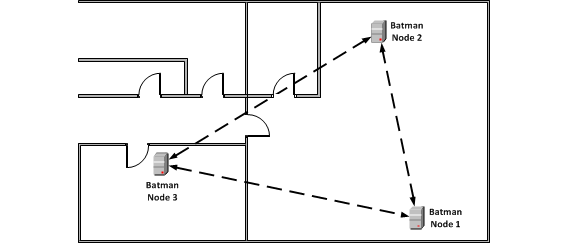
\includegraphics{images/lab_setup_room_view_test1-2.png}
  \caption{Setup for Test I and II.}
  \label{fig:test_1_2}
\end{figure}

\paragraph{Test I} The BATMAN daemon was started on two nodes, node 1 and 2 as shown in Figure \ref{fig:test_1_2}. They where left running until they completed their 4-way handshake and had added each other to their routing tables. The authentication time we used here was the time from when the first OGM is received by the node who becomes the master, until this node has added the other in its routing protocol.

\paragraph{Test II} Two nodes were started like in Test 1. After the network was established and had stabilized, the BATMAN daemon was started on a new node which was then introduced to the network, i.e. node 3 in Figure \ref{fig:test_1_2}. We stopped the test when the new node had been added to the master nodes routing table. The authentication time was the time measured from when the master node received the first OGM from the unauthenticated node until it added the node to its routing protocol.
\\

\begin{figure}[ht!]
  \centering
  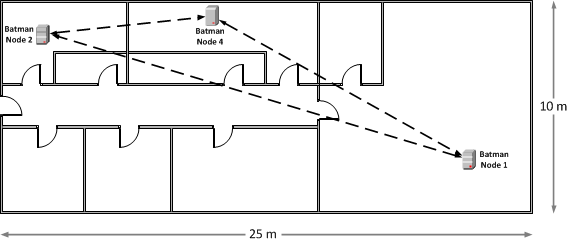
\includegraphics{images/lab_setup_room_view_test3-4.png}
  \caption{Setup for Test III and IV. Node 1 was the master node and the source, and node 2 the sink.}
  \label{fig:test_3_4}
\end{figure}

\paragraph{Test III} A network was established between all of the three nodes as shown in Figure \ref{fig:test_3_4}. When the network was stabilized, node 4 was removed from the preferred path between the source (1) and the sink (2) node.
\\\\
When the source node updated its preferred route to the sink, the test was stopped. The convergence time was measured from when the source node last received a broadcast from node 4, until the source node updated its routing tables accordingly.
\\\\
In order to force the network into believing that the best paths were through node 4, we had to reduce the transmitting power of the source and sink node to 7dBm. To make node 4 disappear and rejoin without re-authentication, we had to set the authentication token value manually in node 4s code, so we could kill the process and restart it bypassing the authentication handshake.

\paragraph{Test IV} When the routing tables had stabilized after the previous test, we reintroduced node 4 to the network. Now we measured the time difference from when the source node first received an OGM from the rejoined node until that node became a part of his preferred route to the sink node again.

\paragraph{Test V} In this test a network of three nodes was established. Once established, the master node was removed and a new unauthenticated node was introduced to the network. After the network had stabilized, we reintroduced the master node and let it start the handshake with the new node. The time measured here was the difference from when the master node first receives an OGM from the network, to the point where the master node adds the new node to its routing tables.
\\\\
Unfortunately, we had problems performing the test V because of time, equipment and laboratory limitations. We were not able to produce several distinct routes with more than three nodes, or else the two different routes would be so much the same that convergence would be in a matter of one or two seconds and not realistic to any real world scenario. And for test V we needed a minimum of four nodes - one sink, one source, one master and one regular node for which both constitutes different routes between the source and the sink. With more time we could have been able to find another way of performing the test.
\\\\
The timestamps used for calculating the authentication and convergence time is found from analyzing the debug output generated while running the BATMAN protocol. The complete logs from the testing can be found in Appendix \ref{appendix_tests}. The results from these tests can be found in the next chapter.
